% Propósito: integrar ITD, ILD y pistas espectrales, y mostrar por qué dos
% números interaurales no resuelven por sí solos todas las posiciones.
% Origen: definiciones de ITD e ILD, modelo
% \eqref{eq:u7-itd-geometrica} y discusión del cono de confusión de las
% secciones \ref{sec:u7-itd-ild}--\ref{sec:u7-pistas-espectrales}.
% Geometría conceptual sin escala ni valores anatómicos.
% Descripción accesible: el panel izquierdo muestra una fuente lateral y dos
% recorridos hacia los oídos; el oído cercano recibe antes y con otro nivel. El
% panel derecho muestra dos fuentes sobre un arco de posiciones que podrían
% compartir ITD e ILD; pabellón y movimiento de cabeza aportan pistas
% espectrales y dinámicas para reducir la ambigüedad.
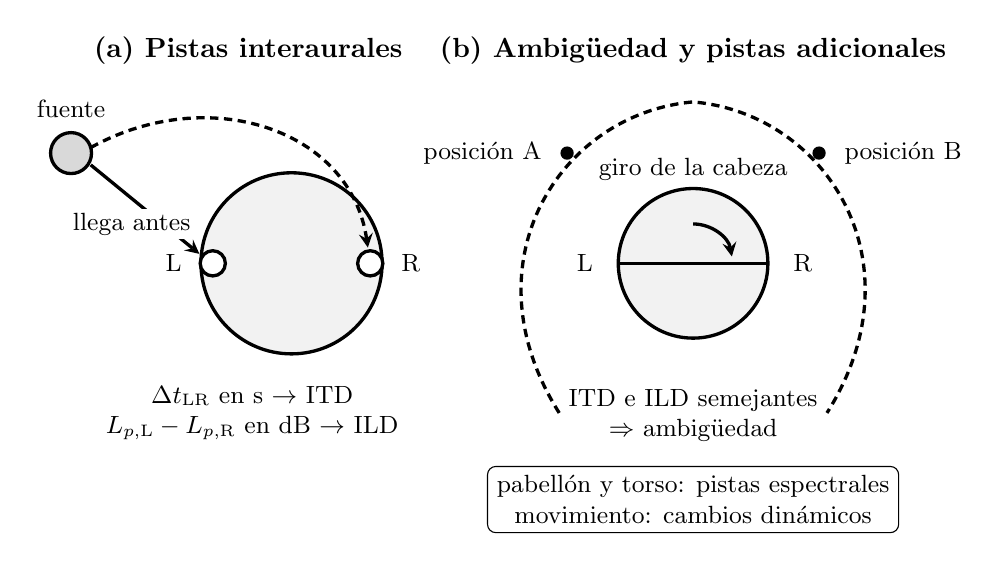
\begin{tikzpicture}[font=\small,>=stealth,x=1cm,y=1cm]
    \node[font=\bfseries] at (3.10,5.45)
        {(a) Pistas interaurales};
    \draw[very thick,fill=black!5] (3.65,2.75) circle (1.15);
    \draw[very thick,fill=white] (2.65,2.75) circle (0.16);
    \draw[very thick,fill=white] (4.65,2.75) circle (0.16);
    \node[anchor=east] at (2.38,2.75) {L};
    \node[anchor=west] at (4.92,2.75) {R};

    \draw[very thick,fill=black!15] (0.85,4.15) circle (0.26);
    \node[anchor=south] at (0.85,4.48) {fuente};
    \draw[->,very thick] (1.10,4.00) -- (2.48,2.87);
    \node[fill=white,inner sep=1.5pt] at (1.62,3.25)
        {llega antes};
    \draw[->,very thick,densely dashed]
        (1.10,4.22) .. controls (2.60,5.05) and (4.40,4.45) .. (4.62,2.95);
    \node[align=center] at (3.15,0.85)
        {\(\Delta t_\mathrm{LR}\) en s \(\rightarrow\) ITD\\
         \(L_{p,\mathrm{L}}-L_{p,\mathrm{R}}\) en dB \(\rightarrow\) ILD};

    \node[font=\bfseries] at (8.75,5.45)
        {(b) Ambigüedad y pistas adicionales};
    \draw[very thick,fill=black!5] (8.75,2.75) circle (0.95);
    \draw[very thick] (7.80,2.75) -- (9.70,2.75);
    \node[anchor=east] at (7.60,2.75) {L};
    \node[anchor=west] at (9.90,2.75) {R};

    \draw[very thick,densely dashed]
        (7.05,0.85) .. controls (5.85,2.75) and (7.05,4.65) ..
        (8.75,4.80) .. controls (10.45,4.65) and (11.65,2.75) ..
        (10.45,0.85);
    \fill (7.15,4.15) circle (2.4pt);
    \fill (10.35,4.15) circle (2.4pt);
    \node[anchor=east,align=right] at (6.95,4.15)
        {posición A};
    \node[anchor=west,align=left] at (10.55,4.15)
        {posición B};
    \node[align=center] at (8.75,0.82)
        {ITD e ILD semejantes\\
         \(\Rightarrow\) ambigüedad};

    \draw[->,very thick]
        (8.75,3.25) arc[start angle=90,end angle=10,radius=0.50];
    \node[align=center,fill=white,inner sep=1.5pt] at (8.75,3.95)
        {giro de la cabeza};
    \node[draw,rounded corners=3pt,align=center,fill=white] at (8.75,-0.25)
        {pabellón y torso: pistas espectrales\\
         movimiento: cambios dinámicos};
\end{tikzpicture}
